% Options for packages loaded elsewhere
\PassOptionsToPackage{unicode}{hyperref}
\PassOptionsToPackage{hyphens}{url}
\PassOptionsToPackage{dvipsnames,svgnames,x11names}{xcolor}
%
\documentclass[
  letterpaper,
  DIV=11,
  numbers=noendperiod]{scrartcl}

\usepackage{amsmath,amssymb}
\usepackage{iftex}
\ifPDFTeX
  \usepackage[T1]{fontenc}
  \usepackage[utf8]{inputenc}
  \usepackage{textcomp} % provide euro and other symbols
\else % if luatex or xetex
  \usepackage{unicode-math}
  \defaultfontfeatures{Scale=MatchLowercase}
  \defaultfontfeatures[\rmfamily]{Ligatures=TeX,Scale=1}
\fi
\usepackage{lmodern}
\ifPDFTeX\else  
    % xetex/luatex font selection
\fi
% Use upquote if available, for straight quotes in verbatim environments
\IfFileExists{upquote.sty}{\usepackage{upquote}}{}
\IfFileExists{microtype.sty}{% use microtype if available
  \usepackage[]{microtype}
  \UseMicrotypeSet[protrusion]{basicmath} % disable protrusion for tt fonts
}{}
\makeatletter
\@ifundefined{KOMAClassName}{% if non-KOMA class
  \IfFileExists{parskip.sty}{%
    \usepackage{parskip}
  }{% else
    \setlength{\parindent}{0pt}
    \setlength{\parskip}{6pt plus 2pt minus 1pt}}
}{% if KOMA class
  \KOMAoptions{parskip=half}}
\makeatother
\usepackage{xcolor}
\setlength{\emergencystretch}{3em} % prevent overfull lines
\setcounter{secnumdepth}{-\maxdimen} % remove section numbering
% Make \paragraph and \subparagraph free-standing
\makeatletter
\ifx\paragraph\undefined\else
  \let\oldparagraph\paragraph
  \renewcommand{\paragraph}{
    \@ifstar
      \xxxParagraphStar
      \xxxParagraphNoStar
  }
  \newcommand{\xxxParagraphStar}[1]{\oldparagraph*{#1}\mbox{}}
  \newcommand{\xxxParagraphNoStar}[1]{\oldparagraph{#1}\mbox{}}
\fi
\ifx\subparagraph\undefined\else
  \let\oldsubparagraph\subparagraph
  \renewcommand{\subparagraph}{
    \@ifstar
      \xxxSubParagraphStar
      \xxxSubParagraphNoStar
  }
  \newcommand{\xxxSubParagraphStar}[1]{\oldsubparagraph*{#1}\mbox{}}
  \newcommand{\xxxSubParagraphNoStar}[1]{\oldsubparagraph{#1}\mbox{}}
\fi
\makeatother


\providecommand{\tightlist}{%
  \setlength{\itemsep}{0pt}\setlength{\parskip}{0pt}}\usepackage{longtable,booktabs,array}
\usepackage{calc} % for calculating minipage widths
% Correct order of tables after \paragraph or \subparagraph
\usepackage{etoolbox}
\makeatletter
\patchcmd\longtable{\par}{\if@noskipsec\mbox{}\fi\par}{}{}
\makeatother
% Allow footnotes in longtable head/foot
\IfFileExists{footnotehyper.sty}{\usepackage{footnotehyper}}{\usepackage{footnote}}
\makesavenoteenv{longtable}
\usepackage{graphicx}
\makeatletter
\def\maxwidth{\ifdim\Gin@nat@width>\linewidth\linewidth\else\Gin@nat@width\fi}
\def\maxheight{\ifdim\Gin@nat@height>\textheight\textheight\else\Gin@nat@height\fi}
\makeatother
% Scale images if necessary, so that they will not overflow the page
% margins by default, and it is still possible to overwrite the defaults
% using explicit options in \includegraphics[width, height, ...]{}
\setkeys{Gin}{width=\maxwidth,height=\maxheight,keepaspectratio}
% Set default figure placement to htbp
\makeatletter
\def\fps@figure{htbp}
\makeatother

\KOMAoption{captions}{tableheading}
\makeatletter
\@ifpackageloaded{caption}{}{\usepackage{caption}}
\AtBeginDocument{%
\ifdefined\contentsname
  \renewcommand*\contentsname{Table of contents}
\else
  \newcommand\contentsname{Table of contents}
\fi
\ifdefined\listfigurename
  \renewcommand*\listfigurename{List of Figures}
\else
  \newcommand\listfigurename{List of Figures}
\fi
\ifdefined\listtablename
  \renewcommand*\listtablename{List of Tables}
\else
  \newcommand\listtablename{List of Tables}
\fi
\ifdefined\figurename
  \renewcommand*\figurename{Figure}
\else
  \newcommand\figurename{Figure}
\fi
\ifdefined\tablename
  \renewcommand*\tablename{Table}
\else
  \newcommand\tablename{Table}
\fi
}
\@ifpackageloaded{float}{}{\usepackage{float}}
\floatstyle{ruled}
\@ifundefined{c@chapter}{\newfloat{codelisting}{h}{lop}}{\newfloat{codelisting}{h}{lop}[chapter]}
\floatname{codelisting}{Listing}
\newcommand*\listoflistings{\listof{codelisting}{List of Listings}}
\makeatother
\makeatletter
\makeatother
\makeatletter
\@ifpackageloaded{caption}{}{\usepackage{caption}}
\@ifpackageloaded{subcaption}{}{\usepackage{subcaption}}
\makeatother

\ifLuaTeX
  \usepackage{selnolig}  % disable illegal ligatures
\fi
\usepackage{bookmark}

\IfFileExists{xurl.sty}{\usepackage{xurl}}{} % add URL line breaks if available
\urlstyle{same} % disable monospaced font for URLs
\hypersetup{
  pdftitle={Modeling Medical Costs Through Regression},
  pdfauthor={Darwhin Gomez},
  colorlinks=true,
  linkcolor={blue},
  filecolor={Maroon},
  citecolor={Blue},
  urlcolor={Blue},
  pdfcreator={LaTeX via pandoc}}


\title{Modeling Medical Costs Through Regression}
\usepackage{etoolbox}
\makeatletter
\providecommand{\subtitle}[1]{% add subtitle to \maketitle
  \apptocmd{\@title}{\par {\large #1 \par}}{}{}
}
\makeatother
\subtitle{CUNY SPS DATA 621}
\author{Darwhin Gomez}
\date{}

\begin{document}
\maketitle

\renewcommand*\contentsname{Table of contents}
{
\hypersetup{linkcolor=}
\setcounter{tocdepth}{3}
\tableofcontents
}

Medical costs represent a significant financial burden for individuals
and are a primary reason health insurance coverage is widely sought.
Accurately understanding the factors that drive medical insurance
charges is essential for insurers seeking to price plans fairly and
sustainably, as well as for policymakers concerned with healthcare
affordability. This paper aims to model the relationship between
individual medical insurance costs and selected demographic,
health-related, and behavioral indicators using linear regression
techniques. Using a dataset of insured individuals in the United States,
we examine how factors such as age, body mass index (BMI), smoking
status, number of dependents, and geographic region influence medical
charges. Multiple regression models are developed and evaluated to
identify statistically significant predictors and assess model
assumptions. The results provide interpretable insights into the primary
drivers of medical insurance costs and demonstrate the usefulness of
regression modeling in health economics and insurance pricing
applications.

\subsection{\texorpdfstring{\textbf{Abstract}}{Abstract}}\label{abstract}

Medical insurance costs are highly variable, right-skewed, and
influenced by both demographic and behavioral factors. Accurately
modeling these costs is essential for insurers seeking to price risk
fairly and sustainably. This study examines the relationship between
medical insurance charges and individual characteristics using
regression-based approaches. Using a dataset of 1,338 insured
individuals in the United States, we evaluate ordinary least squares
regression, interaction models, robust regression, and generalized
linear models. Due to the skewed and heteroskedastic nature of cost
data, a Gamma generalized linear model with a log link and selected
interaction terms was chosen as the final specification. Results
indicate that smoking status is the dominant driver of medical costs and
significantly amplifies the effect of body mass index. The final model
demonstrates strong predictive performance on a held-out test set and
provides interpretable insights relevant for insurance pricing and risk
assessment.

\subsection{\texorpdfstring{\textbf{1.
Introduction}}{1. Introduction}}\label{introduction}

Rising healthcare costs present a significant financial challenge for
individuals, insurers, and policymakers. Medical insurance premiums are
typically based on expected healthcare utilization, which in turn
depends on demographic characteristics, health indicators, and
behavioral risk factors. Understanding how these factors jointly
influence medical costs is critical for effective risk pricing and
sustainable insurance design.

Traditional linear regression models are often used to analyze cost data
due to their interpretability; however, medical costs violate many
classical regression assumptions. Costs are strictly positive,
right-skewed, and characterized by a small number of high-cost
individuals who account for a disproportionate share of total
expenditures. As a result, naïve linear regression may produce biased
inference and poor predictive performance.

This study addresses these challenges by applying regression techniques
tailored to cost data. Specifically, we investigate whether smoking
status modifies the effects of other predictors---particularly body mass
index---on medical insurance charges. The objective is twofold: (1) to
identify key drivers of medical costs and (2) to develop a predictive
model that balances interpretability with statistical appropriateness.

\subsection{\texorpdfstring{\textbf{2. Literature
Review}}{2. Literature Review}}\label{literature-review}

Modeling healthcare expenditures presents significant econometric
challenges due to the inherently skewed and heavy-tailed nature of cost
data. Medical expenditures are characterized by a large mass of low-cost
observations and a long right tail of extremely high costs. These
features are commonly associated with heteroscedastic error structures,
leading to frequent violations of the homoscedasticity assumption in
ordinary least squares regression.

A common response is to apply a logarithmic transformation to costs and
estimate a linear model on the transformed scale. However, this approach
introduces important limitations. Zero-cost observations cannot be
accommodated without ad hoc adjustments, and retransformation bias
arises when predicted log-costs are exponentiated to recover expected
costs on the original scale. As shown by Manning (1998), this bias
persists under heteroscedasticity, which is common even after log
transformation. While smearing estimators may partially address this
issue (Duan, 1983; Duan et al., 1983), they rely on additional
assumptions and do not fully resolve model misspecification (Manning,
1998).

Generalized linear models provide a more appropriate framework for
modeling healthcare costs (Blough et al., 1999; Deb \& Trivedi, 2002).
By allowing the response variable to follow a distribution from the
exponential dispersion family, GLMs explicitly accommodate the skewed
and heteroscedastic nature of cost data (Glick et al., 2014). In
particular, the Gamma distribution with a log link is well suited for
continuous, positive expenditures, as it naturally models variance
proportional to the square of the mean and ensures positive predictions
(Blough et al., 1999; Deb \& Trivedi, 2002). Coefficients from such
models admit a straightforward multiplicative interpretation in terms of
percentage changes in expected cost (Glick et al., 2014).

Consistent with prior literature, our analysis highlights smoking status
as a dominant cost driver and demonstrates that its effect interacts
strongly with body mass index. This finding aligns with evidence that
health risk factors operate synergistically rather than independently
(Manning et al., 1987; Deb \& Trivedi, 2002). Age and family structure
also exhibit significant relationships with medical expenditures,
reflecting systematic differences in healthcare utilization documented
in prior studies (Blough et al., 1999; Glick et al., 2014).

Overall, the use of a Gamma generalized linear model with targeted
interaction terms aligns with best practices in health econometrics,
yielding consistent estimates and improved efficiency relative to
misspecified linear models (Manning, 1998; Blough et al., 1999; Deb \&
Trivedi, 2002).

\subsection{\texorpdfstring{\textbf{3.
Methodology}}{3. Methodology}}\label{methodology}

\subsubsection{\texorpdfstring{\textbf{3.1 Data}}{3.1 Data}}\label{data}

The dataset is found from the online Data Science community Kaggle.com.
A link to the exact download source is provided in the Appendix.

The dataset consists of 1,338 individuals covered by medical insurance
in the United States. The response variable is annual medical insurance
charges. Predictor variables include age, sex, body mass index (BMI),
smoking status, number of dependents (recoded as a binary indicator for
having children), and residential region.

All variables were complete with no missing observations. Categorical
predictors were encoded as factor variables prior to model estimation.
The number of children was originally measured as a numeric variable and
was subsequently recoded as a binary indicator reflecting the presence
of dependents.

\subsubsection{\texorpdfstring{\textbf{3.2 Exploratory
Analysis}}{3.2 Exploratory Analysis}}\label{exploratory-analysis}

Exploratory data analysis revealed that medical charges are heavily
right-skewed, with a long upper tail corresponding to high-cost
individuals. Boxplots and residual diagnostics confirmed the presence of
heteroskedasticity and non-normality, consistent with the known
characteristics of healthcare cost data. These patterns motivated the
use of modeling approaches beyond ordinary least squares regression.

\subsubsection{\texorpdfstring{\textbf{3.3 Model
Specification}}{3.3 Model Specification}}\label{model-specification}

\textbf{Several models were estimated and compared:}

Ordinary least squares regression on raw charges

Linear regression with interaction terms

Robust regression to assess sensitivity to outliers

Gamma generalized linear models with a log link

To assess effect heterogeneity, interaction terms between smoking status
and other predictors were explored. While smoking significantly modified
the effects of BMI, age, and dependent status, interactions with sex and
region did not materially improve model fit.

The final model specification was a \textbf{Gamma generalized linear
model with a log link} including the following predictors: Age, BMI,
Smoking status,Having children, Sex, Region, Smoking × BMI, Smoking,
Age, Smoking × Having children

\subsubsection{\texorpdfstring{\textbf{3.4 Model
Evaluation}}{3.4 Model Evaluation}}\label{model-evaluation}

The dataset was split into training (70\%) and testing (30\%) subsets.
Model performance was evaluated on the test set using root mean squared
error (RMSE) and mean absolute error (MAE), with predictions generated
on the original cost scale using the inverse log link.

\subsection{\texorpdfstring{\textbf{4.
Results}}{4. Results}}\label{results}

The final Gamma model demonstrated strong explanatory power, reducing
deviance substantially relative to a null model and achieving a
deviance-based pseudo-R² of approximately 0.73.

Smoking status emerged as the dominant predictor of medical costs.
Holding other factors constant, smokers incur nearly three times the
expected medical costs of non-smokers. Body mass index alone had little
effect among non-smokers; however, for smokers, each additional BMI unit
increased expected medical costs by approximately 5\%. This interaction
indicates that smoking substantially amplifies the cost impact of
obesity.

Age was also a significant predictor, with expected medical costs
increasing by roughly 3--4\% per additional year for non-smokers. The
interaction between smoking and age suggested that the marginal effect
of age is attenuated among smokers, likely reflecting their already
elevated baseline risk. Having dependents increased expected costs for
non-smokers, though this effect was weaker among smokers.

On the held-out test set, the model achieved an RMSE of approximately
\$5,200 and an MAE of approximately \$3,170. A predicted-versus-actual
plot showed good calibration across most of the cost distribution, with
increased dispersion among very high-cost individuals.

\subsection{\texorpdfstring{\textbf{5.
Discussion}}{5. Discussion}}\label{discussion}

The results highlight smoking as the most influential driver of medical
insurance costs, both directly and through its interaction with BMI and
age. From a business perspective, these findings support risk-adjusted
pricing strategies that account not only for smoking status but also for
how smoking interacts with other health indicators.

The strong interaction between smoking and BMI suggests that wellness
interventions targeting weight management among smokers may yield
disproportionately large cost savings. Insurers may also benefit from
differentiated premium structures or targeted preventive care programs
for high-risk subgroups identified by the model.

\subsection{\texorpdfstring{\textbf{6.
Limitations}}{6. Limitations}}\label{limitations}

Several limitations should be noted. The dataset does not include
detailed clinical variables such as diagnosed conditions or healthcare
utilization patterns, which likely explain much of the remaining
variation in high-cost cases. Additionally, the analysis focuses on
expected costs rather than extreme tail risk, which may be of interest
for reinsurance or catastrophic coverage modeling.

\subsection{\texorpdfstring{\textbf{7.
Conclusion}}{7. Conclusion}}\label{conclusion}

This study demonstrates that medical insurance costs can be effectively
modeled using regression-based approaches when the distributional
characteristics of cost data are properly addressed. A Gamma generalized
linear model with targeted interaction terms provides a robust,
interpretable framework for understanding cost drivers and predicting
expected medical expenditures. The findings underscore the central role
of \textbf{smoking} in healthcare costs and illustrate the value of
interaction modeling in uncovering meaningful risk heterogeneity.

\begin{figure}[H]

{\centering 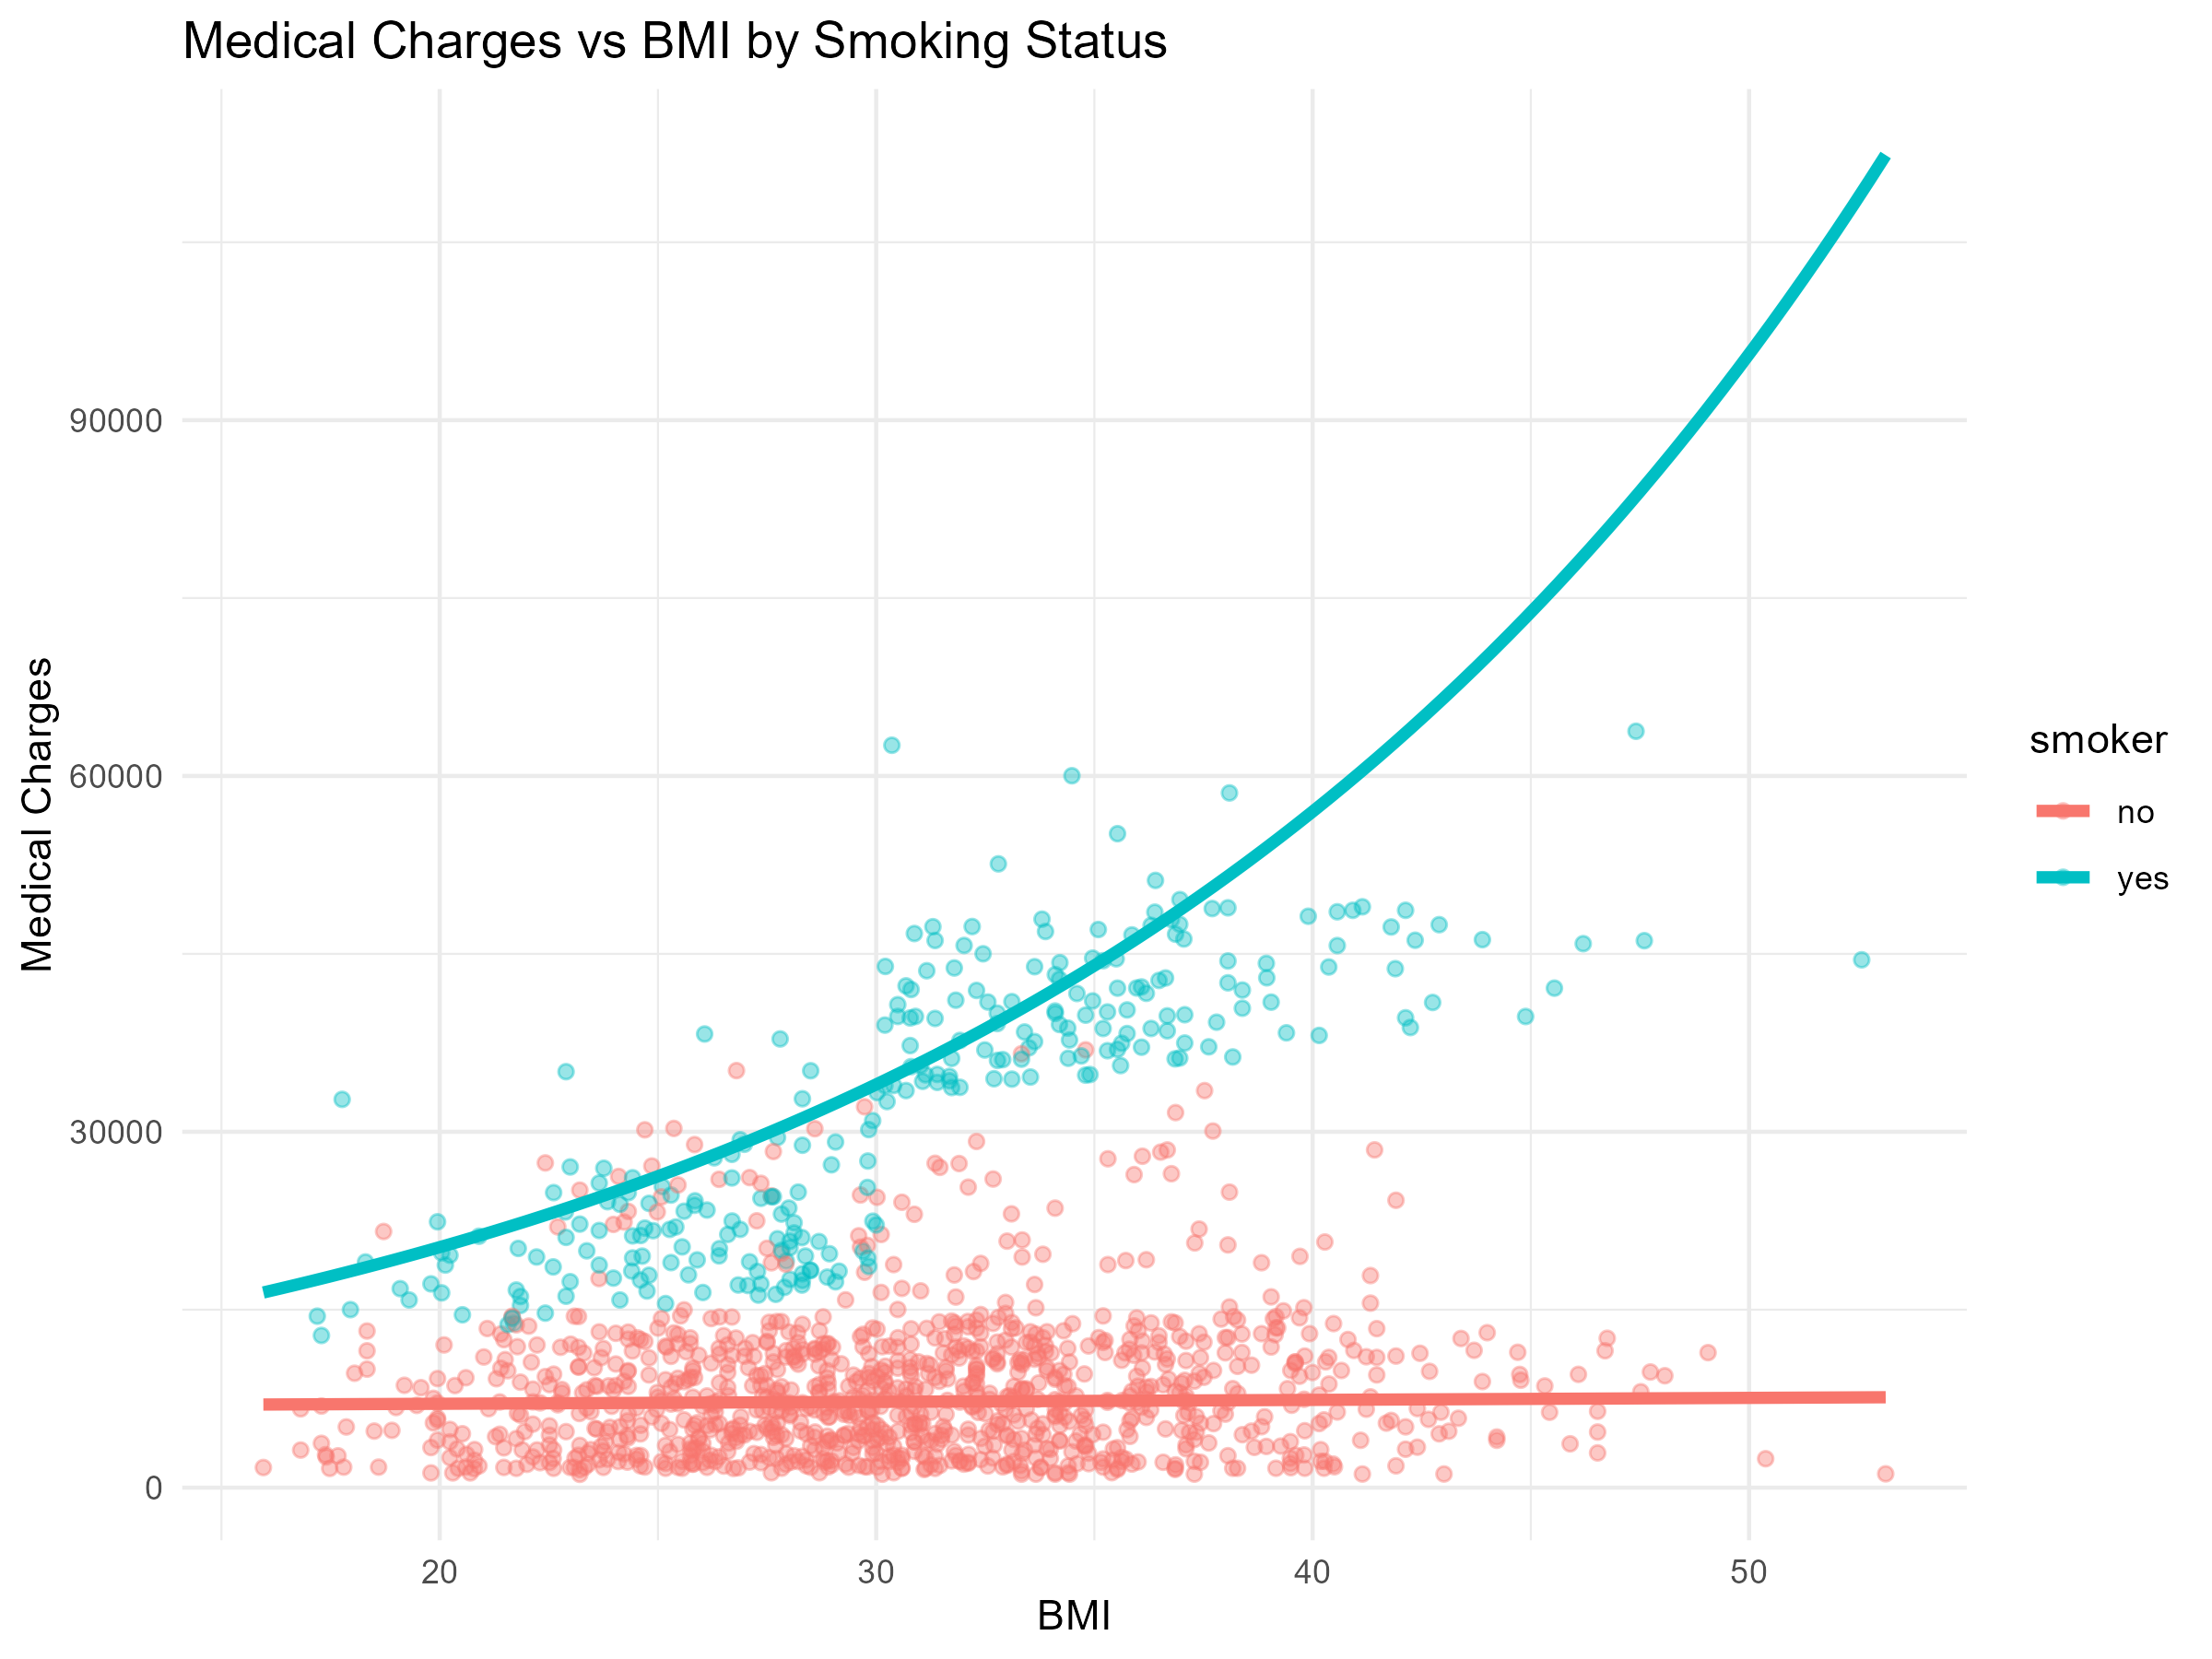
\includegraphics[width=6.25in,height=\textheight]{plots/bmi_charges_gamma_glm_fit.png}

}

\caption{GLM BMI Smoker}

\end{figure}%

Medical insurance charges as a function of body mass index (BMI),
stratified by smoking status. Points represent observed charges, while
solid lines represent fitted values from the final Gamma generalized
linear model with a log link and interaction between BMI and smoking
status. Predicted values are shown on the original cost scale.

\begin{verbatim}
The mdoel's rmse: 5198.975  The models mae 3170.379
\end{verbatim}

\subsection{Appendices}\label{appendices}

\subsubsection{Tables and Figures}\label{tables-and-figures}

\subsubsection{Models}\label{models}

\begin{verbatim}

Call:
lm(formula = charges ~ ., data = data_clean)

Residuals:
     Min       1Q   Median       3Q      Max 
-11483.5  -2894.7   -956.5   1478.1  30059.6 

Coefficients:
                 Estimate Std. Error t value Pr(>|t|)    
(Intercept)     -12001.01     993.99 -12.074  < 2e-16 ***
age                256.91      11.92  21.562  < 2e-16 ***
sexmale           -126.41     333.31  -0.379  0.70456    
bmi                339.51      28.63  11.858  < 2e-16 ***
smokeryes        23849.65     413.63  57.660  < 2e-16 ***
regionnorthwest   -352.22     476.88  -0.739  0.46029    
regionsoutheast  -1057.33     479.27  -2.206  0.02755 *  
regionsouthwest   -944.26     478.40  -1.974  0.04861 *  
has_childrenYes    999.58     335.88   2.976  0.00297 ** 
---
Signif. codes:  0 '***' 0.001 '**' 0.01 '*' 0.05 '.' 0.1 ' ' 1

Residual standard error: 6069 on 1329 degrees of freedom
Multiple R-squared:  0.7503,    Adjusted R-squared:  0.7488 
F-statistic: 499.3 on 8 and 1329 DF,  p-value: < 2.2e-16
\end{verbatim}

\begin{verbatim}

Call:
lm(formula = charges ~ bmi * smoker + age + has_children, data = data_clean)

Residuals:
     Min       1Q   Median       3Q      Max 
-14992.4  -2033.6  -1242.8   -372.9  29880.8 

Coefficients:
                  Estimate Std. Error t value Pr(>|t|)    
(Intercept)      -2753.520    838.589  -3.284 0.001052 ** 
bmi                  6.423     24.950   0.257 0.796894    
smokeryes       -20082.183   1659.601 -12.101  < 2e-16 ***
age                265.192      9.585  27.667  < 2e-16 ***
has_childrenYes    960.640    270.224   3.555 0.000391 ***
bmi:smokeryes     1430.143     52.987  26.991  < 2e-16 ***
---
Signif. codes:  0 '***' 0.001 '**' 0.01 '*' 0.05 '.' 0.1 ' ' 1

Residual standard error: 4886 on 1332 degrees of freedom
Multiple R-squared:  0.8378,    Adjusted R-squared:  0.8372 
F-statistic:  1376 on 5 and 1332 DF,  p-value: < 2.2e-16
\end{verbatim}

\begin{verbatim}

Call:
lm(formula = sqrt(charges) ~ (bmi * smoker + age), data = data_clean)

Residuals:
    Min      1Q  Median      3Q     Max 
-32.971  -9.796  -4.530   0.831 107.572 

Coefficients:
               Estimate Std. Error t value Pr(>|t|)    
(Intercept)    28.14841    3.49594   8.052 1.79e-15 ***
bmi             0.05813    0.10529   0.552    0.581    
smokeryes     -31.44669    7.00376  -4.490 7.74e-06 ***
age             1.43666    0.04041  35.554  < 2e-16 ***
bmi:smokeryes   3.97785    0.22361  17.789  < 2e-16 ***
---
Signif. codes:  0 '***' 0.001 '**' 0.01 '*' 0.05 '.' 0.1 ' ' 1

Residual standard error: 20.62 on 1333 degrees of freedom
Multiple R-squared:  0.8142,    Adjusted R-squared:  0.8137 
F-statistic:  1461 on 4 and 1333 DF,  p-value: < 2.2e-16
\end{verbatim}

\subparagraph{Selected Model}\label{selected-model}

\begin{verbatim}

Call:
glm(formula = charges ~ age + bmi + has_children + sex + region + 
    smoker + smoker:bmi + smoker:age + smoker:has_children, family = Gamma(link = "log"), 
    data = data_clean)

Coefficients:
                           Estimate Std. Error t value Pr(>|t|)    
(Intercept)                7.467355   0.127288  58.665  < 2e-16 ***
age                        0.034462   0.001534  22.466  < 2e-16 ***
bmi                        0.002258   0.003690   0.612  0.54075    
has_childrenYes            0.270674   0.043227   6.262 5.13e-10 ***
sexmale                   -0.063918   0.038358  -1.666  0.09588 .  
regionnorthwest           -0.066977   0.054828  -1.222  0.22208    
regionsoutheast           -0.151504   0.055130  -2.748  0.00608 ** 
regionsouthwest           -0.169059   0.055015  -3.073  0.00216 ** 
smokeryes                  1.080839   0.266440   4.057 5.27e-05 ***
bmi:smokeryes              0.049428   0.007595   6.508 1.08e-10 ***
age:smokeryes             -0.025914   0.003422  -7.573 6.78e-14 ***
has_childrenYes:smokeryes -0.274594   0.096193  -2.855  0.00438 ** 
---
Signif. codes:  0 '***' 0.001 '**' 0.01 '*' 0.05 '.' 0.1 ' ' 1

(Dispersion parameter for Gamma family taken to be 0.4861963)

    Null deviance: 1056.04  on 1337  degrees of freedom
Residual deviance:  288.82  on 1326  degrees of freedom
AIC: 26168

Number of Fisher Scoring iterations: 6
\end{verbatim}

\subsubsection{Exploratory Plots}\label{exploratory-plots}

\begin{figure}[H]

{\centering 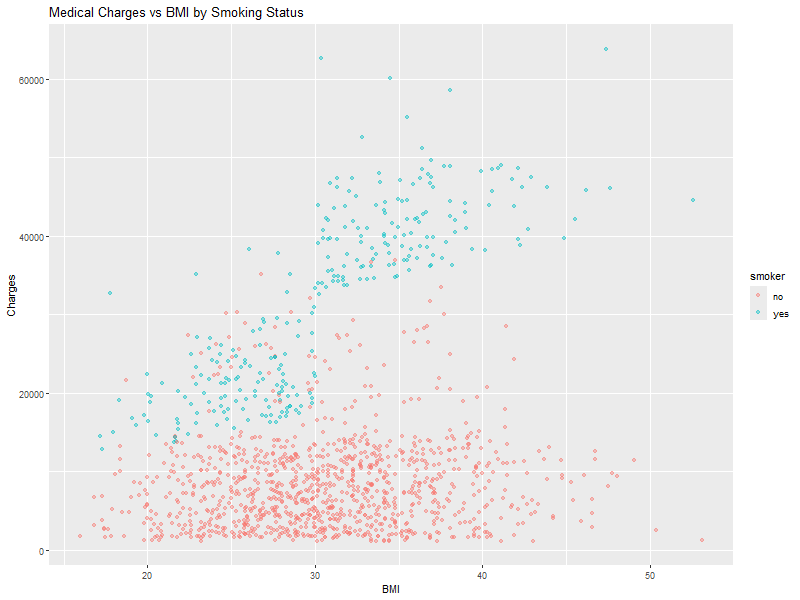
\includegraphics[width=6.25in,height=\textheight]{plots/scatter_bmi_charges.png}

}

\caption{Cost and BMI Smoker Labels}

\end{figure}%%
\begin{figure}[H]

{\centering 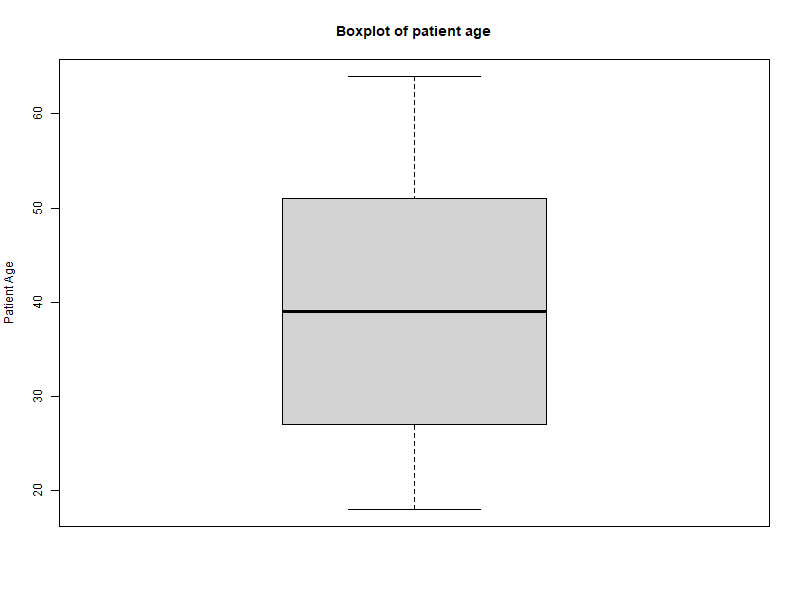
\includegraphics[width=6.375in,height=\textheight]{plots/boxplot_age.png}

}

\caption{Box Plot - Age}

\end{figure}%%
\begin{figure}[H]

{\centering 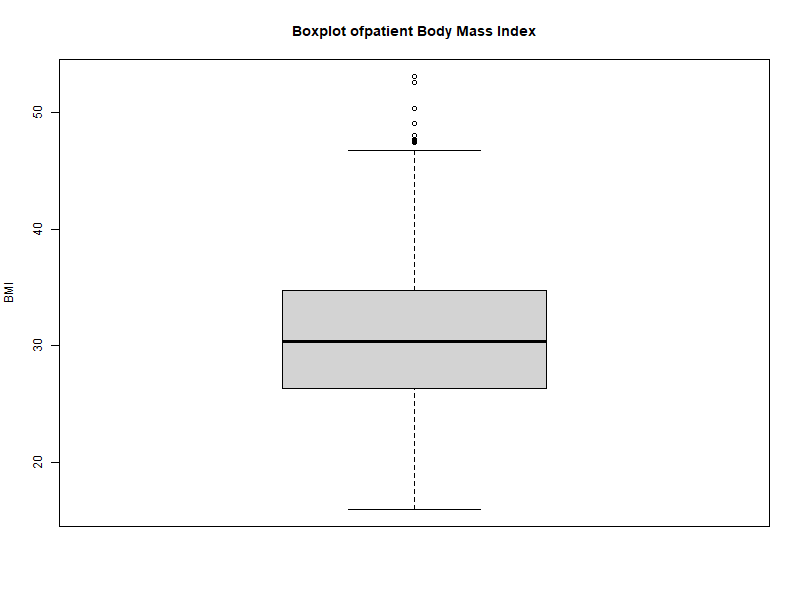
\includegraphics[width=6.375in,height=\textheight]{plots/boxplot_bmi.png}

}

\caption{Box Plot - Body Mass Index}

\end{figure}%%
\begin{figure}[H]

{\centering 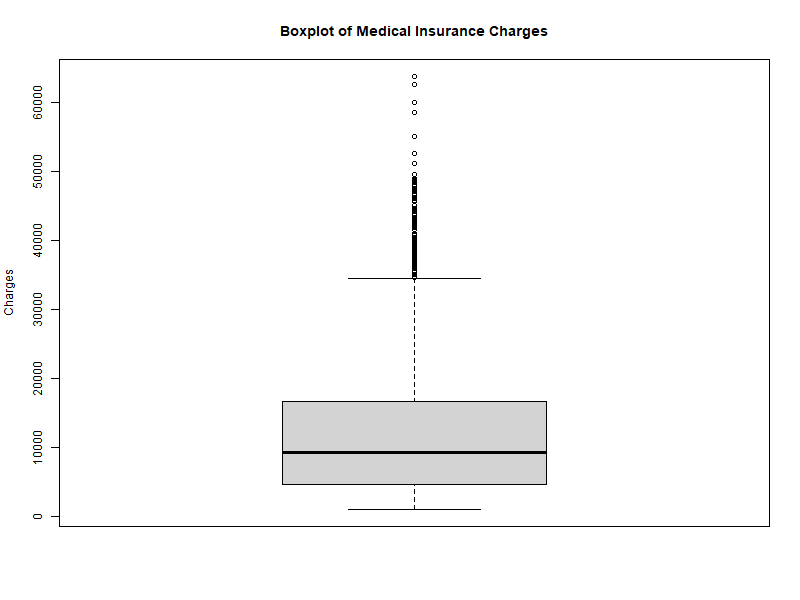
\includegraphics[width=6.375in,height=\textheight]{plots/boxplot_charges.png}

}

\caption{Box Plot- Charges}

\end{figure}%%
\begin{figure}[H]

{\centering 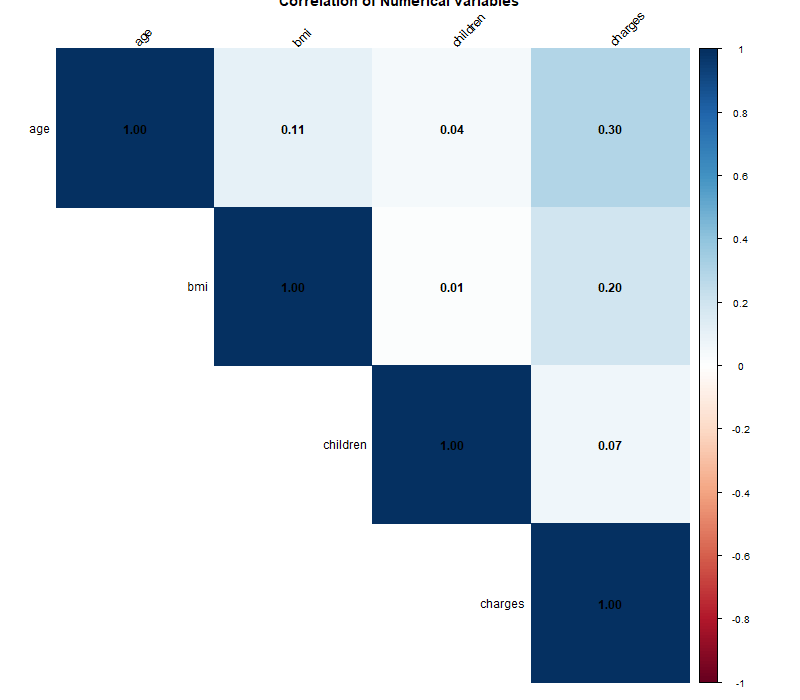
\includegraphics[width=5.46875in,height=\textheight]{plots/correlation_matrix.png}

}

\caption{Numerical Correlation To Target}

\end{figure}%%
\begin{figure}[H]

{\centering 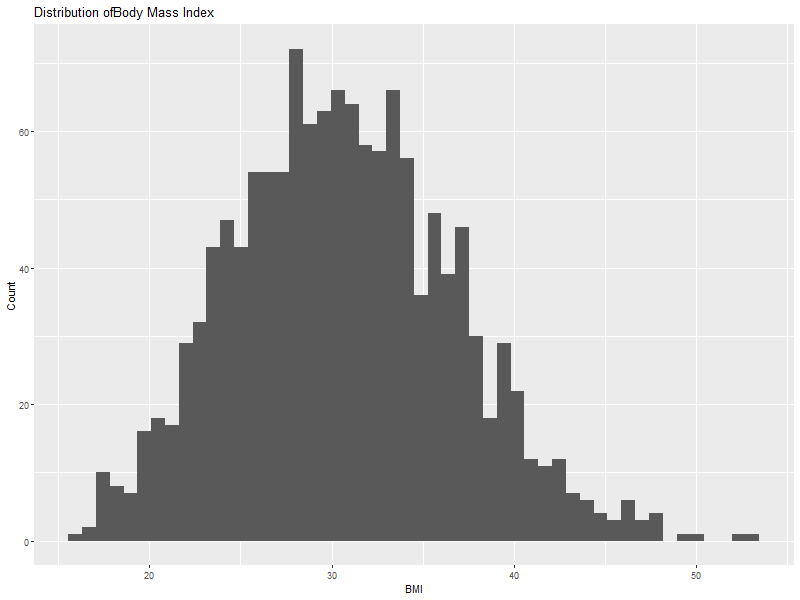
\includegraphics[width=6.375in,height=\textheight]{plots/distribution_Bmi.png}

}

\caption{Distribution - BMI}

\end{figure}%%
\begin{figure}[H]

{\centering 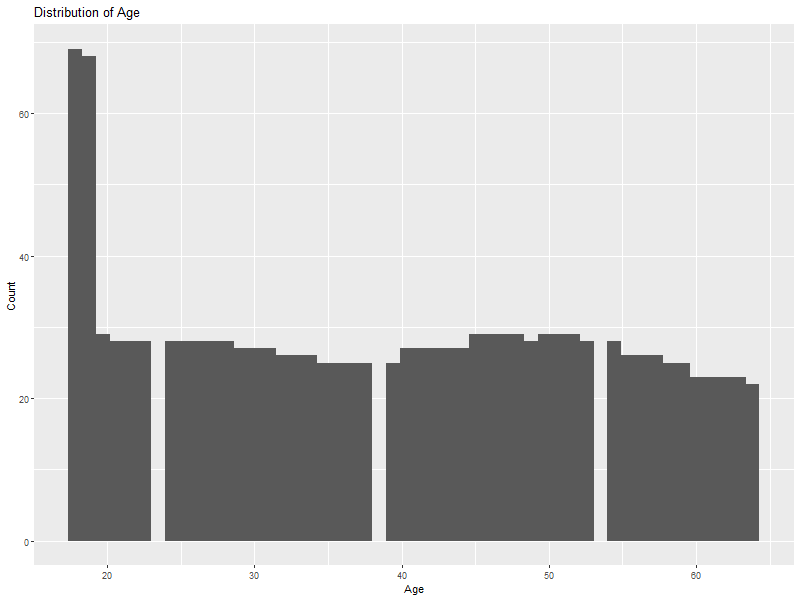
\includegraphics[width=6.375in,height=\textheight]{plots/distribution_age.png}

}

\caption{Distribution - Age}

\end{figure}%%
\begin{figure}[H]

{\centering 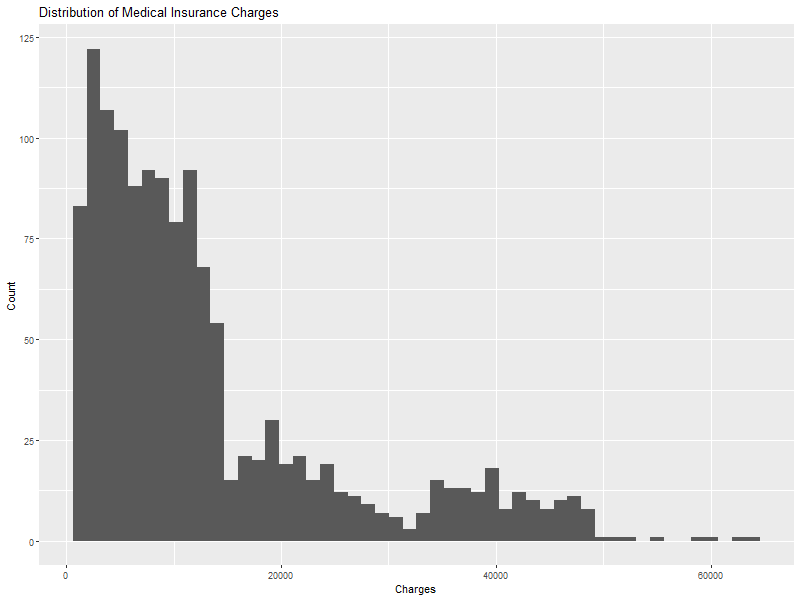
\includegraphics[width=6.375in,height=\textheight]{plots/distribution_target.png}

}

\caption{Distribution - Charges}

\end{figure}%

\subsubsection{Model Diagnostic Plots}\label{model-diagnostic-plots}

\begin{figure}[H]

{\centering 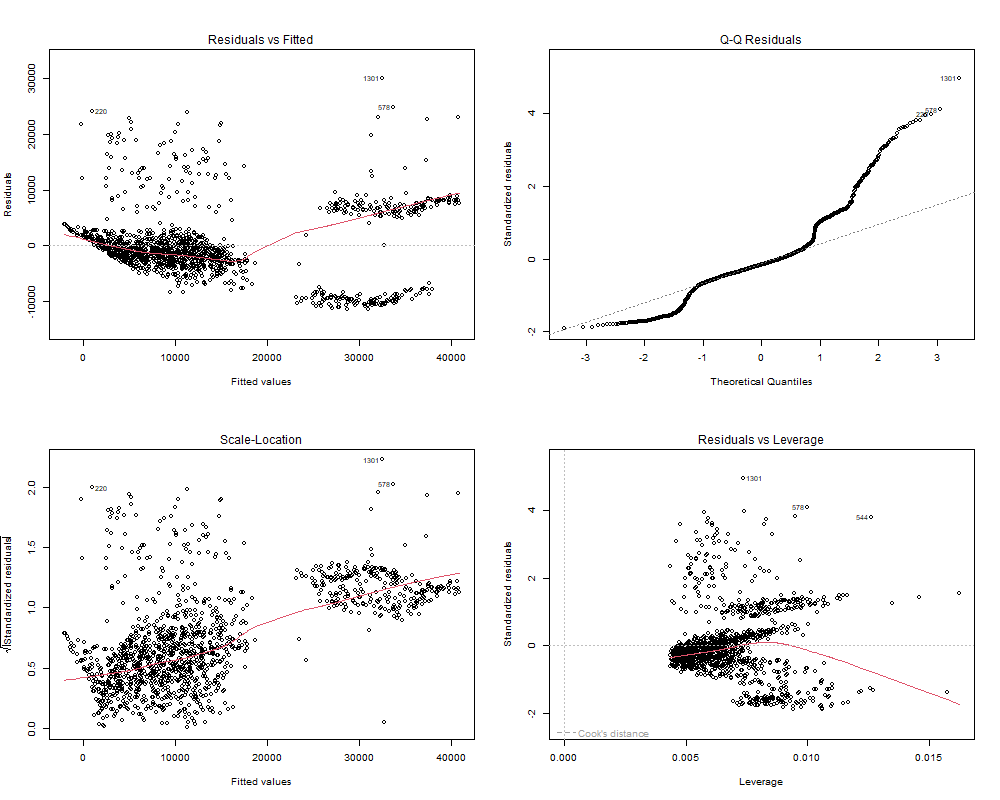
\includegraphics[width=6.375in,height=\textheight]{plots/linear_model_diagnostics.png}

}

\caption{Linear model Diagnostics}

\end{figure}%%
\begin{figure}[H]

{\centering 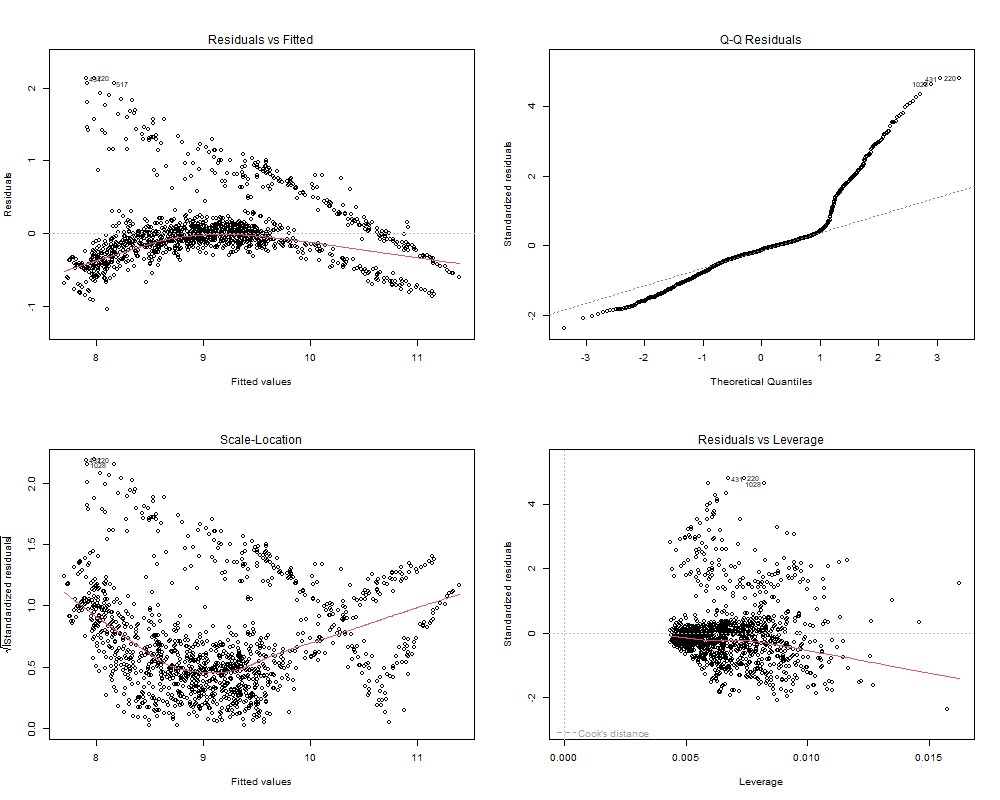
\includegraphics[width=6.375in,height=\textheight]{plots/log_linear_model_diagnostics.png}

}

\caption{Log Linear Model Diagnostics}

\end{figure}%%
\begin{figure}[H]

{\centering 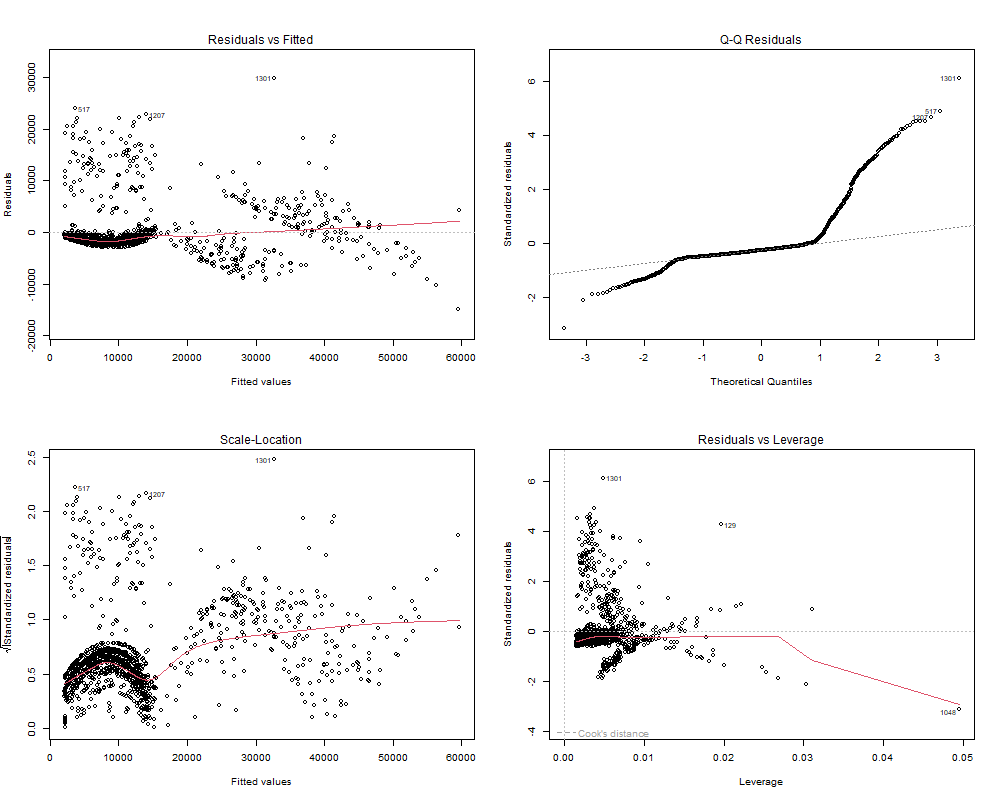
\includegraphics[width=6.375in,height=\textheight]{plots/interaction_model_diagnostics.png}

}

\caption{Interaction Linear Model Smoker * BMI}

\end{figure}%

\paragraph{Model Selected}\label{model-selected}

\begin{figure}[H]

{\centering 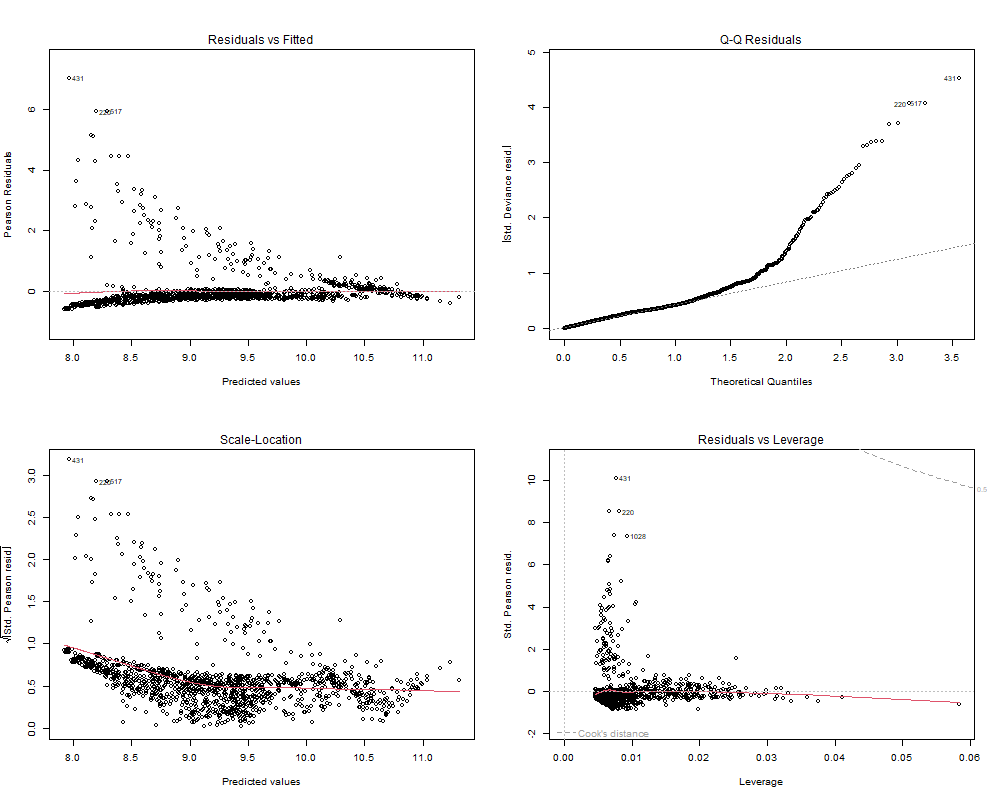
\includegraphics[width=6.375in,height=\textheight]{plots/gamma_final_model_diagnostics.png}

}

\caption{GLM Final Model}

\end{figure}%%
\begin{figure}[H]

{\centering 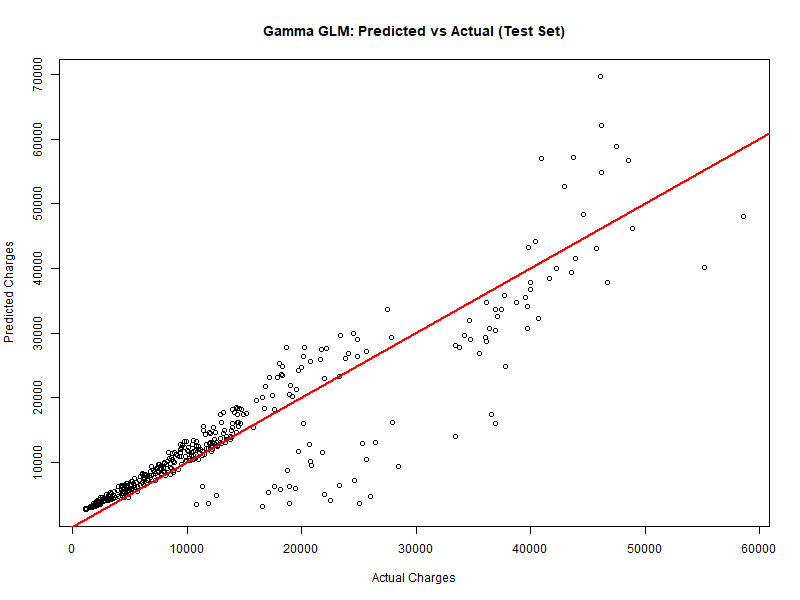
\includegraphics[width=6.375in,height=\textheight]{plots/gamma_pred_vs_actual.png}

}

\caption{Actual V Predicted}

\end{figure}%%
\begin{figure}[H]

{\centering 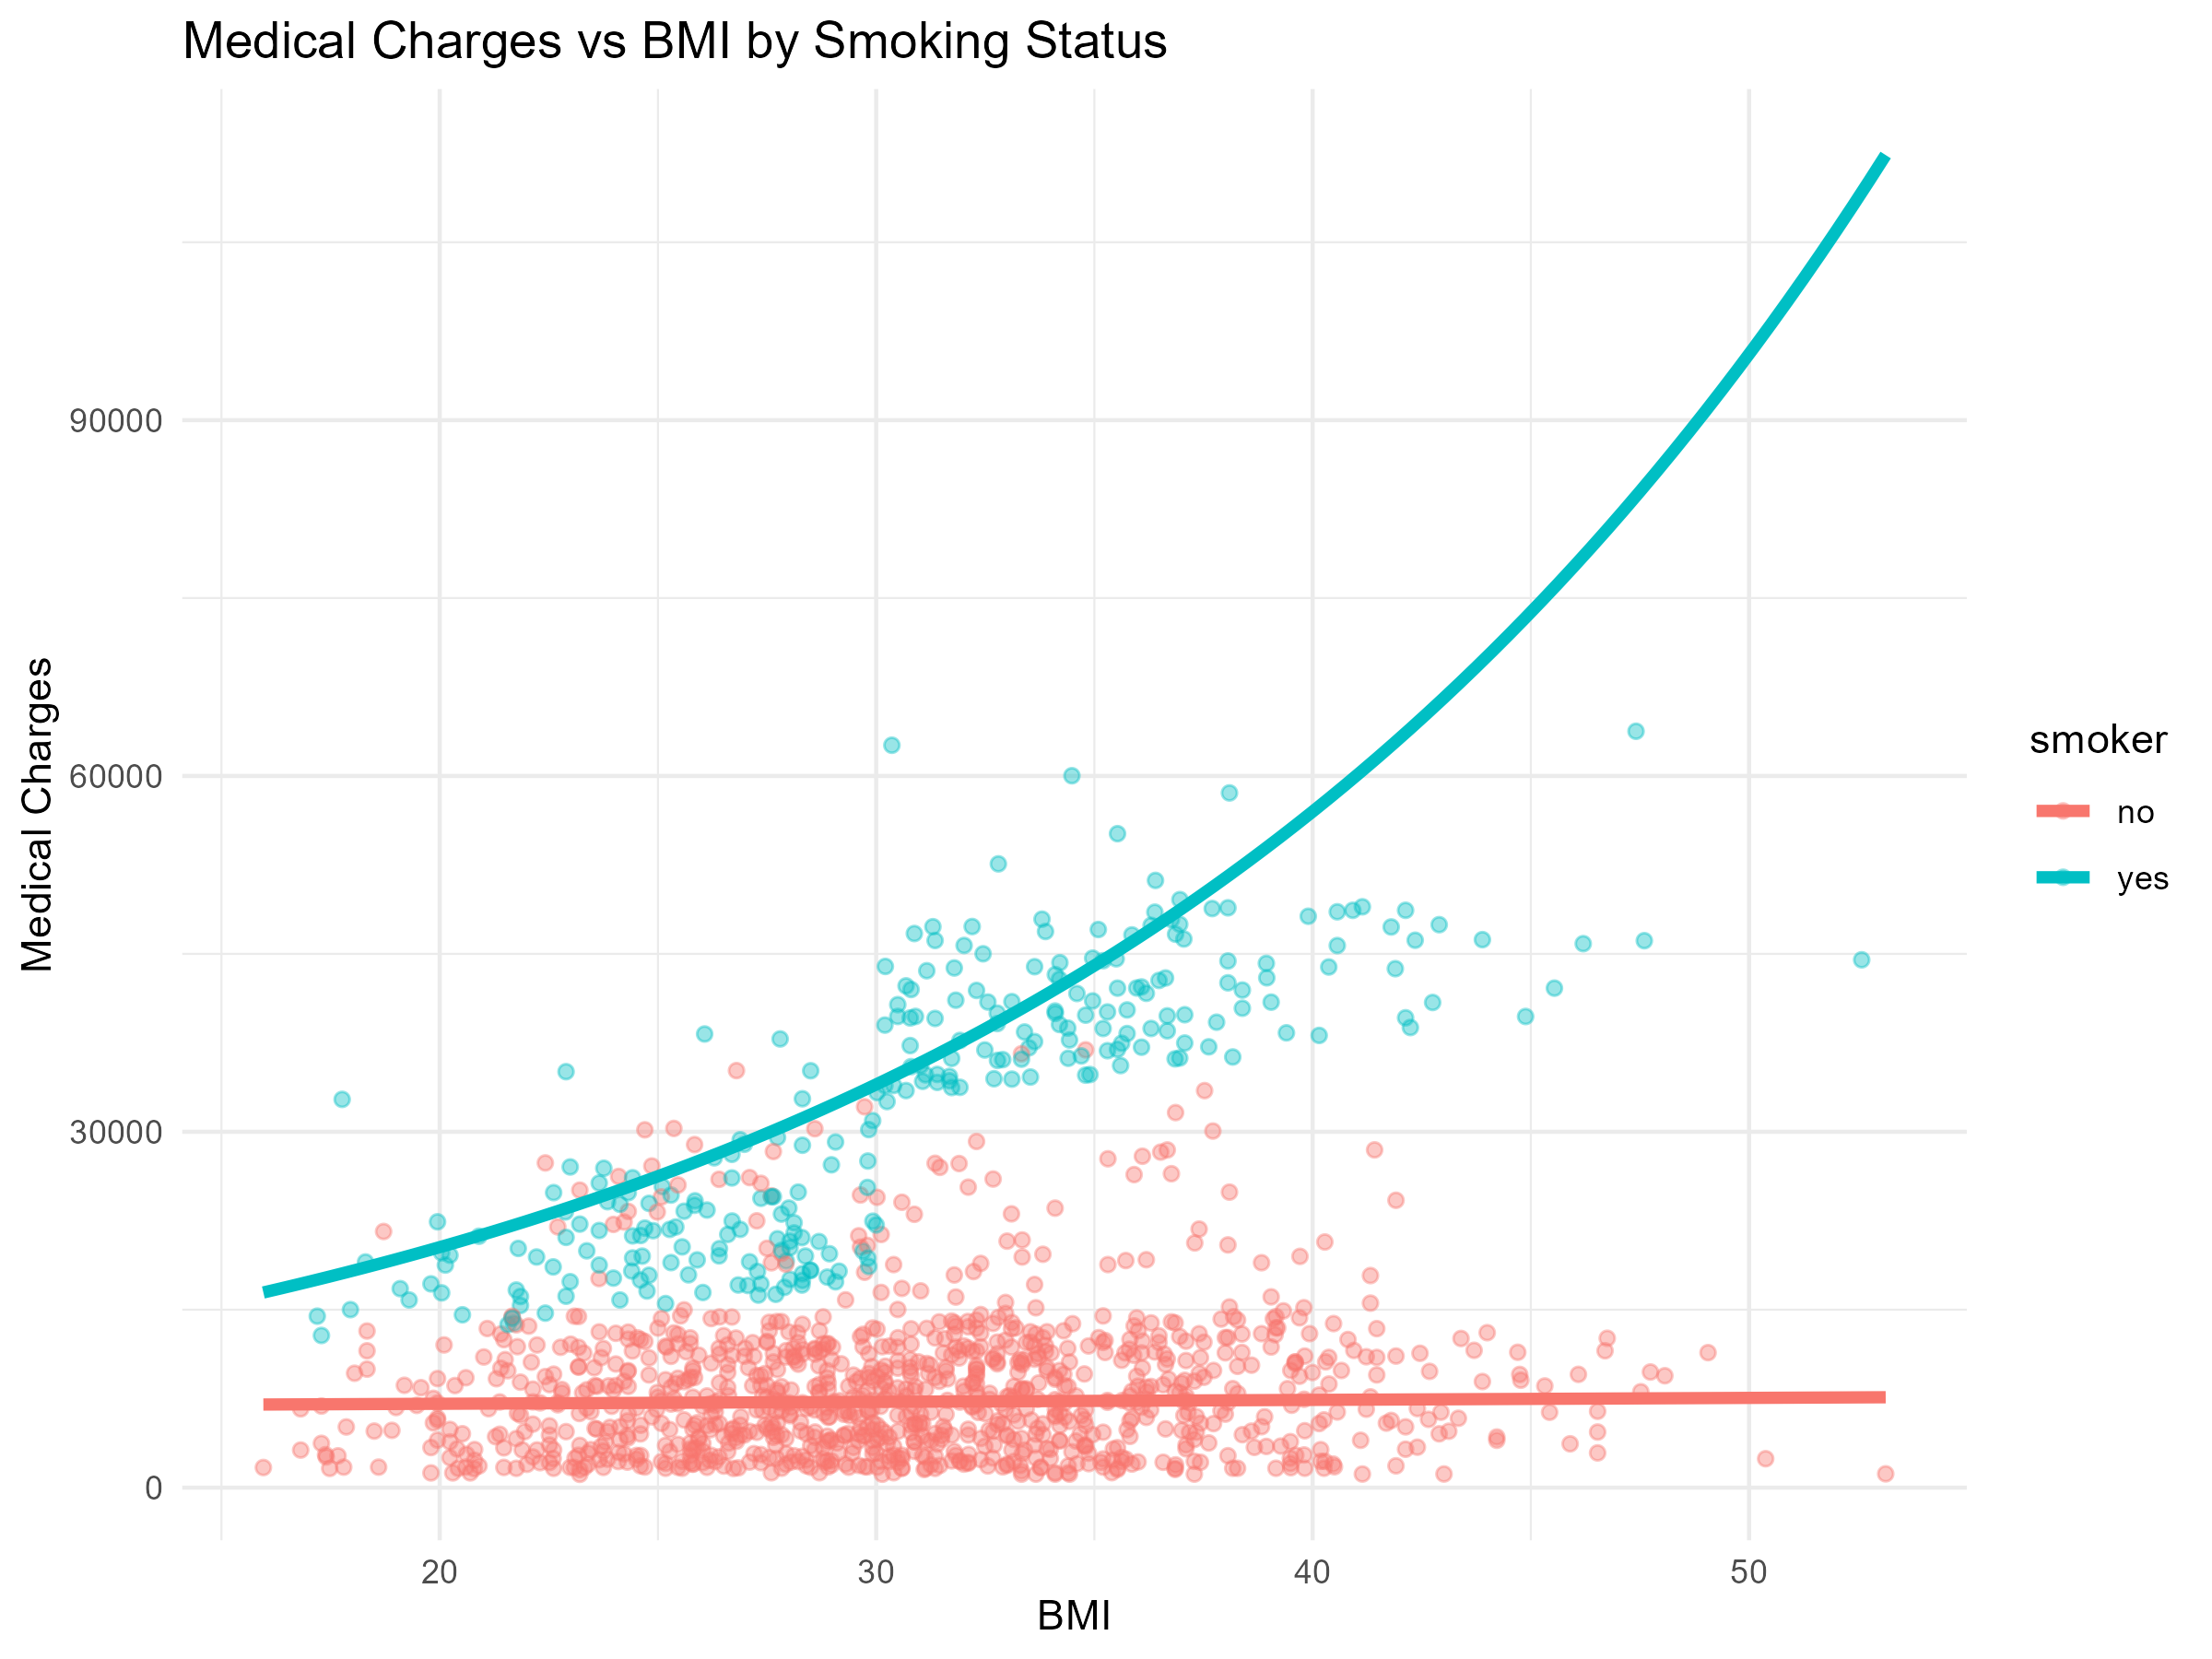
\includegraphics[width=6.25in,height=\textheight]{plots/bmi_charges_gamma_glm_fit.png}

}

\caption{BMI Smoker GLM}

\end{figure}%

\subsubsection{References}\label{references}

Manning, W. G. (1998). The logged dependent variable,
heteroscedasticity, and the retransformation problem. \emph{Journal of
Health Economics, 17}(3), 283--295.
https://doi.org/10.1016/S0167-6296(98)00025-3

Blough, D. K., Madden, C. W., \& Hornbrook, M. C. (1999). Modeling risk
using generalized linear models. \emph{Journal of Health Economics,
18}(2), 153--171. https://doi.org/10.1016/S0167-6296(98)00041-1

Deb, P., \& Trivedi, P. K. (2002). The structure of demand for health
care by the elderly: Econometric evidence from the Health and Retirement
Study. \emph{Journal of Health Economics, 21}(5), 803--824.
https://doi.org/10.1016/S0167-6296(02)00021-7

Glick, H. A., Doshi, J. A., Sonnad, S. S., \& Polsky, D. (2014).
\emph{Economic evaluation in clinical trials} (2nd ed.). Oxford
University Press.

\paragraph{Data}\label{data-1}

Abdelghany, M. (2025). \emph{Medical insurance cost dataset} {[}Data
set{]}. Kaggle. \url{https://doi.org/10.34740/KAGGLE/DSV/12853160}

\subsubsection{R Code}\label{r-code}

\href{https://github.com/DW8888/data621/blob/main/FinalProject/analysis.Rmd}{R
code Link}

\subsubsection{Predictions}\label{predictions}

\begin{verbatim}
    Predicted charges
1           21667.670
2            5038.960
3            4639.096
4            4122.332
5           29303.890
6            3309.855
7           15008.039
8           35764.482
9           15374.077
10           3453.264
11          43254.124
12           7563.904
13           4722.729
14          18232.641
15          18171.631
16          20064.448
17          14671.339
18           5725.687
19           3152.160
20           7242.559
21           8996.259
22          39299.724
23           8503.573
24          11575.900
25          10236.835
26          15330.048
27           3975.315
28           4082.238
29           9001.299
30           3220.740
31           3480.834
32          35483.043
33           3130.432
34           3720.357
35           3419.793
36          20478.467
37           5846.825
38          25659.763
39           5846.385
40          32297.263
41           3729.171
42          24713.371
43          33711.791
44          11759.760
45          34723.498
46          12776.781
47          11585.490
48           6965.176
49           4436.735
50          13583.932
51           8033.744
52          10091.537
53          12085.888
54           3049.048
55           4804.498
56          57151.096
57           5421.165
58           3538.956
59           3166.220
60          17356.019
61          13921.274
62           9793.813
63           5167.157
64           3623.992
65          11718.099
66          29035.963
67           4035.101
68          16036.034
69           2960.915
70           3498.093
71           6241.120
72          16166.321
73          41529.979
74           6099.973
75          27709.145
76          26419.087
77          54772.624
78           9172.891
79           3866.868
80           6440.580
81           9584.883
82          23015.811
83          34746.569
84           7918.280
85           5574.483
86           5894.672
87          26843.127
88          56742.537
89          13599.835
90          18141.460
91           3596.394
92           3146.587
93           4423.483
94           7200.641
95           9965.981
96           6503.324
97           4239.782
98          13308.270
99          14046.840
100         13119.523
101         25362.868
102         25954.463
103         10115.530
104          7262.874
105          2883.653
106         12122.143
107         12042.383
108          9214.050
109          3120.227
110          8976.342
111         16000.059
112         15013.187
113          7185.584
114         21295.282
115         15603.567
116          3410.133
117         18334.933
118          4913.227
119          6100.487
120         12517.132
121          3763.969
122          6479.874
123         13148.691
124         32620.192
125          3341.873
126         11522.443
127         27578.707
128         11990.163
129          6360.497
130          3870.823
131          3851.262
132          9531.281
133         10893.413
134         46164.010
135          3483.270
136          7662.204
137          7796.128
138          4236.471
139          3859.879
140         11089.481
141         10427.555
142         10954.087
143         11479.932
144         14028.825
145          4219.745
146         10568.079
147         26050.287
148         37767.908
149          3201.730
150         11266.741
151          6110.268
152         17672.584
153         47964.989
154         17410.496
155          6264.738
156          2795.826
157          7827.168
158         10625.523
159          6347.110
160          8959.510
161         14013.510
162         19540.276
163         27123.798
164          7762.654
165          3507.005
166         23232.261
167          5485.110
168         11000.312
169         31933.766
170         12515.015
171          6346.780
172         52600.604
173         12246.816
174         11524.444
175         16239.518
176          4364.064
177         26440.784
178         13745.311
179         14503.806
180          5128.654
181          8814.707
182         13391.784
183          8436.238
184         12438.585
185         10493.044
186         36798.494
187         43000.292
188          5584.397
189          5100.489
190          6626.366
191         62153.607
192         13580.717
193          6297.897
194          6151.934
195          3600.765
196          9961.443
197          4759.045
198         10844.973
199          9624.108
200         11584.839
201          6506.011
202         11646.411
203         10119.098
204          3556.025
205         11699.757
206          2890.171
207         11847.040
208         12755.827
209         12558.742
210         44230.821
211         10712.304
212         23628.389
213          3103.690
214          5308.774
215          4346.560
216         21896.021
217          9874.117
218          8794.058
219         14668.694
220         16134.489
221          8930.916
222         10179.478
223          2878.786
224          6129.669
225          3440.502
226          2839.720
227          3935.700
228          8840.701
229         24862.980
230         23107.288
231          3940.617
232          8366.667
233          9349.060
234          3421.122
235          5399.116
236         12468.616
237          5942.402
238          6911.615
239          4365.245
240         29623.213
241         40122.446
242          9245.661
243          9605.961
244         12823.894
245          8106.882
246         13097.682
247          5998.925
248          7510.882
249          8528.811
250         12850.292
251          8080.127
252          3066.482
253         29249.870
254         33680.362
255          4577.770
256         11002.150
257         17715.896
258         26784.153
259          3147.475
260         69684.126
261          8512.293
262          2853.872
263         14300.164
264          4843.401
265          8560.028
266          7410.493
267          4195.532
268          5059.101
269         24285.941
270          7278.700
271         11143.693
272          4103.520
273          3062.709
274          5606.430
275         12647.804
276          9660.987
277         20417.253
278          4578.860
279         17405.785
280          3713.274
281         12888.910
282          7114.699
283          6429.207
284         12960.834
285         14453.080
286          8207.225
287          5032.439
288          6059.125
289         12011.489
290          2764.579
291         12254.692
292         58812.648
293          4888.774
294          4256.307
295         13123.284
296          9708.068
297          8168.276
298         11768.525
299          5956.519
300          3743.975
301          5560.207
302         20230.398
303          4588.617
304         18286.786
305         11653.883
306          9270.388
307          8022.143
308          3360.030
309         28953.375
310         13283.566
311         17394.932
312         11318.753
313          4762.498
314          8738.167
315         39951.595
316         13701.631
317         34136.002
318          4119.393
319         27691.623
320         28035.041
321          4111.198
322         15507.412
323         30673.409
324          4356.023
325          5575.594
326         18529.496
327         15452.301
328          3589.969
329         17495.247
330          3612.261
331         11754.378
332         12362.150
333          4578.455
334         48394.852
335          5038.204
336         18275.063
337         10376.614
338         12750.563
339          9130.038
340         13250.046
341         28716.735
342          6258.094
343         56979.174
344          7141.252
345          2966.267
346         12819.080
347         10237.145
348         30421.248
349         11264.167
350          8565.498
351         12695.240
352         13115.022
353         11947.389
354          8338.360
355          6564.420
356          8292.702
357         23117.378
358          7964.396
359          5878.260
360          3353.081
361         12758.564
362         23432.951
363         33713.098
364         14924.821
365         27389.933
366          6723.463
367          7609.264
368          6999.639
369         16006.883
370         12533.446
371         38435.757
372          8508.315
373          6777.903
374          9330.905
375          6725.493
376         10504.062
377         12973.073
378         15944.054
379         14581.824
380         16112.323
381         12872.568
382          3059.668
383         27756.090
384          2790.151
385          6844.843
386          9120.913
387         10535.917
388         29585.583
389         10427.464
390          5272.620
391         29968.411
392          3238.056
393         37765.224
394          4805.280
395         24825.793
396          8027.887
397          6461.406
398         30672.450
399          6210.509
400          3520.365
401          3039.221
402          3230.003
\end{verbatim}




\end{document}
